\section{Discussion}

In this study we found that Purkinje cells that are close to each other show firing profiles significantly more correlated than cells that are distant. We also showed that during modulation, neighboring cells consistently express correlated firing at short time scales (<5ms), that are not explained by the increase in firing rate.
The correlated firing profiles suggest that the groups of neighboring cells that we record are likely to belong to the same microzone. Thus, our results indicate that cerebellar cortex produces very transient events of inhibition of their postsynaptic targets during movement.

These results are to be examined in the context of the debate about coding in cerebellar cortex. As discussed in the introduction, it is still unclear through which mechanism Purkinje cells control the output of neurons in the deep cerebellar nuclei. The traditional theory suggests that this happens through rate coding, that is Purkinje cells modulate the activity of DCN neurons by their rate of firing. This theory predicts anticorrelation in the activity of the cerebellar cortex and the cerebellar nuclei, but this is not the case. Instead, it has been consistently observed that the DCN neurons correlate both positively and negatively with the activity of Purkinje cells.
This observation contradicts the prediction of the rate hypothesis, while it reinforces the idea of synchrony coding. In fact, the theory of synchrony coding proposes that Purkinje cells control cerebellar nuclei by synchronizing their spikes. This provides control of the cerebellar output because synchronous inhibitory post-synaptic potentials caused by synchronous spikes create periods of time where the DCN cells are prevented from spiking.

The problem with rate coding is that it is very difficult to test. In fact, it would require simultaneous recordings from groups of Purkinje cells and from the DCN cells that receive their synapses, which is unfeasible for with the current technologies. Moreover, to obtain scientific proof and not just observations, we would need a paradigm where synchrony is the independent variable, but we do not know any way to ``desynchronize'' neurons yet. However, models show that synchrony coding could achieve millisecond-scale control of the DCN output \cite{person2012synchrony}, and our results indicate that synchronous spikes are not caused by an increase in firing rate. Since synchrony is not just a secondary effect of enhanced activity, and it allows a control of DCN at the time scale needed to explain behavioral results, synchrony coding looks like a consistent theory on the way Purkinje cells control the DCN output, even if it isn't yet proved.

Another open question is how synchrony between Purkinje cells is achieved: different alternatives are possible, for example \emph{ephatic coupling} \cite{han2018ephaptic}, which allows neurons to communicate through extracellular electrical signals. Ephatic coupling happens because when a neuron has an action potential it reduces the positive charge of the extracellular matrix, and this causes neighboring neurons to be more likely to spike, because their membrane potential difference has been reduced. This mechanism, together with electrical coupling, would explain the high level of sub-millisecond synchrony that other studies have recorded. We didn't observe that kind of synchrony because our spike sorting algorithm could not separate near-coincident spikes, but our results suggest that other mechanisms should be employed to explain more delayed events, for example recurrent connections between Purkinje cells \cite{de2008high}.

The mechanisms responsible for the Purkinje cells synchronization described in our results are currently undetermined. Multiple candidate mechanisms have been described \cite{person2012synchrony} (Figure \ref{fig:clem}), including electrical coupling between Purkinje cells (causing with excitatory spikelets in neighboring cells), shared excitation from parallel fibers or climbing fibers, ephaptic coupling (change in membrane potential due to a change in extracellular potential caused by the action potential of a neighboring cell) between the Purkinje cells, and recurrent inhibition via collaterals between Purkinje neurons. According to the literature, the electrical and ephaptic coupling more likely result in synchrony at the millisecond scale so are unlikely to be the cause of the effect described in our work. The climbing fibers fire at a frequency of ~1Hz, so the spike induced by this afferent represent only 1-5\% of the spikes and are therefore unlikely causing the 20\% excess synchrony that we observed. Finally, the shared parallel fibers and the recurrent inhibition are the most likely cause of synchrony in our system. Disentangling the role of these two mechanisms would probably remain very challenging experimentally.

Ultimately, our results add more evidence in favor of the theory of synchrony coding, but they don't prove that synchronous activity of Purkinje cells is actually the mechanism that enables control on the neurons in the cerebellar nuclei. Also, we cannot be sure that the neighboring neurons are actually part of the same microzone, since the synapses that they make with climbing fibers are very hard to trace back to the olivar neurons.

Evidence of significant small time scale synchronization should probably discourage the use of imaging methods for the study of cerebellar cortex. In fact, even if the last advances suggest that calcium imaging allows identification of single spikes, the delay of activation of calcium markers - which is on the order of tens of milliseconds - would probably work against a precise quantification of co-activation.  

\begin{figure}[H]
  \centering
  % \fbox{
% \parbox[c]{\textwidth}{
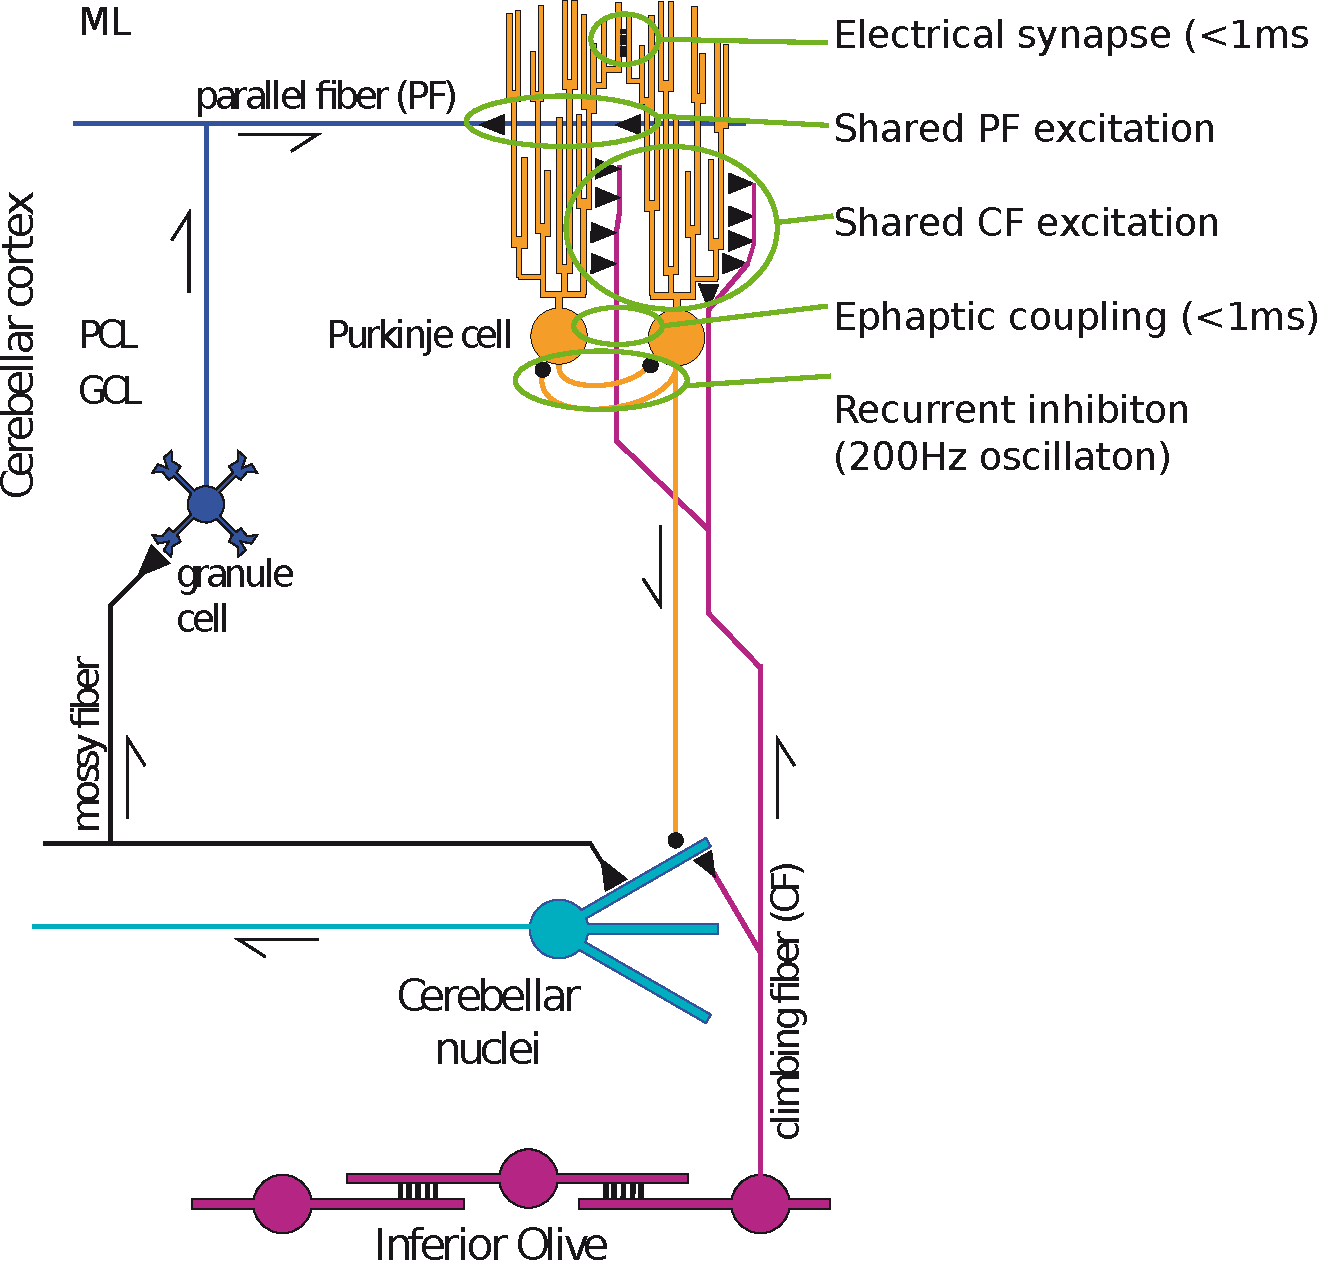
\includegraphics[scale=0.4]{schemaSync.pdf}
\caption{
\textbf{Anatomy and functionality of the cerebellar cortex}\\
ML: molecular layer, PCL: Purkinje cells layer, GCL: granular cells layer, PF: parallel fibers, CF: climbing fibers}
  \label{fig:clem}%}}
\end{figure}
